\documentclass{article}
\usepackage[english]{babel}
\usepackage[letterpaper,top=2cm,bottom=2cm,left=3cm,right=3cm,marginparwidth=1.75cm]{geometry}

\usepackage{amsmath}
\usepackage{graphicx}
% add graphics path
\graphicspath{{./graph/}}
\usepackage{indentfirst}
\usepackage{amsfonts}
\usepackage{caption}
\usepackage[colorlinks=true, allcolors=blue]{hyperref}

\usepackage{upgreek}

\title{Assignment 2}
\author{Shuhao Bian}

\begin{document}
\maketitle

\section{Problem 1}

% insert a pdf here
\begin{figure}[h!]
    \centering
    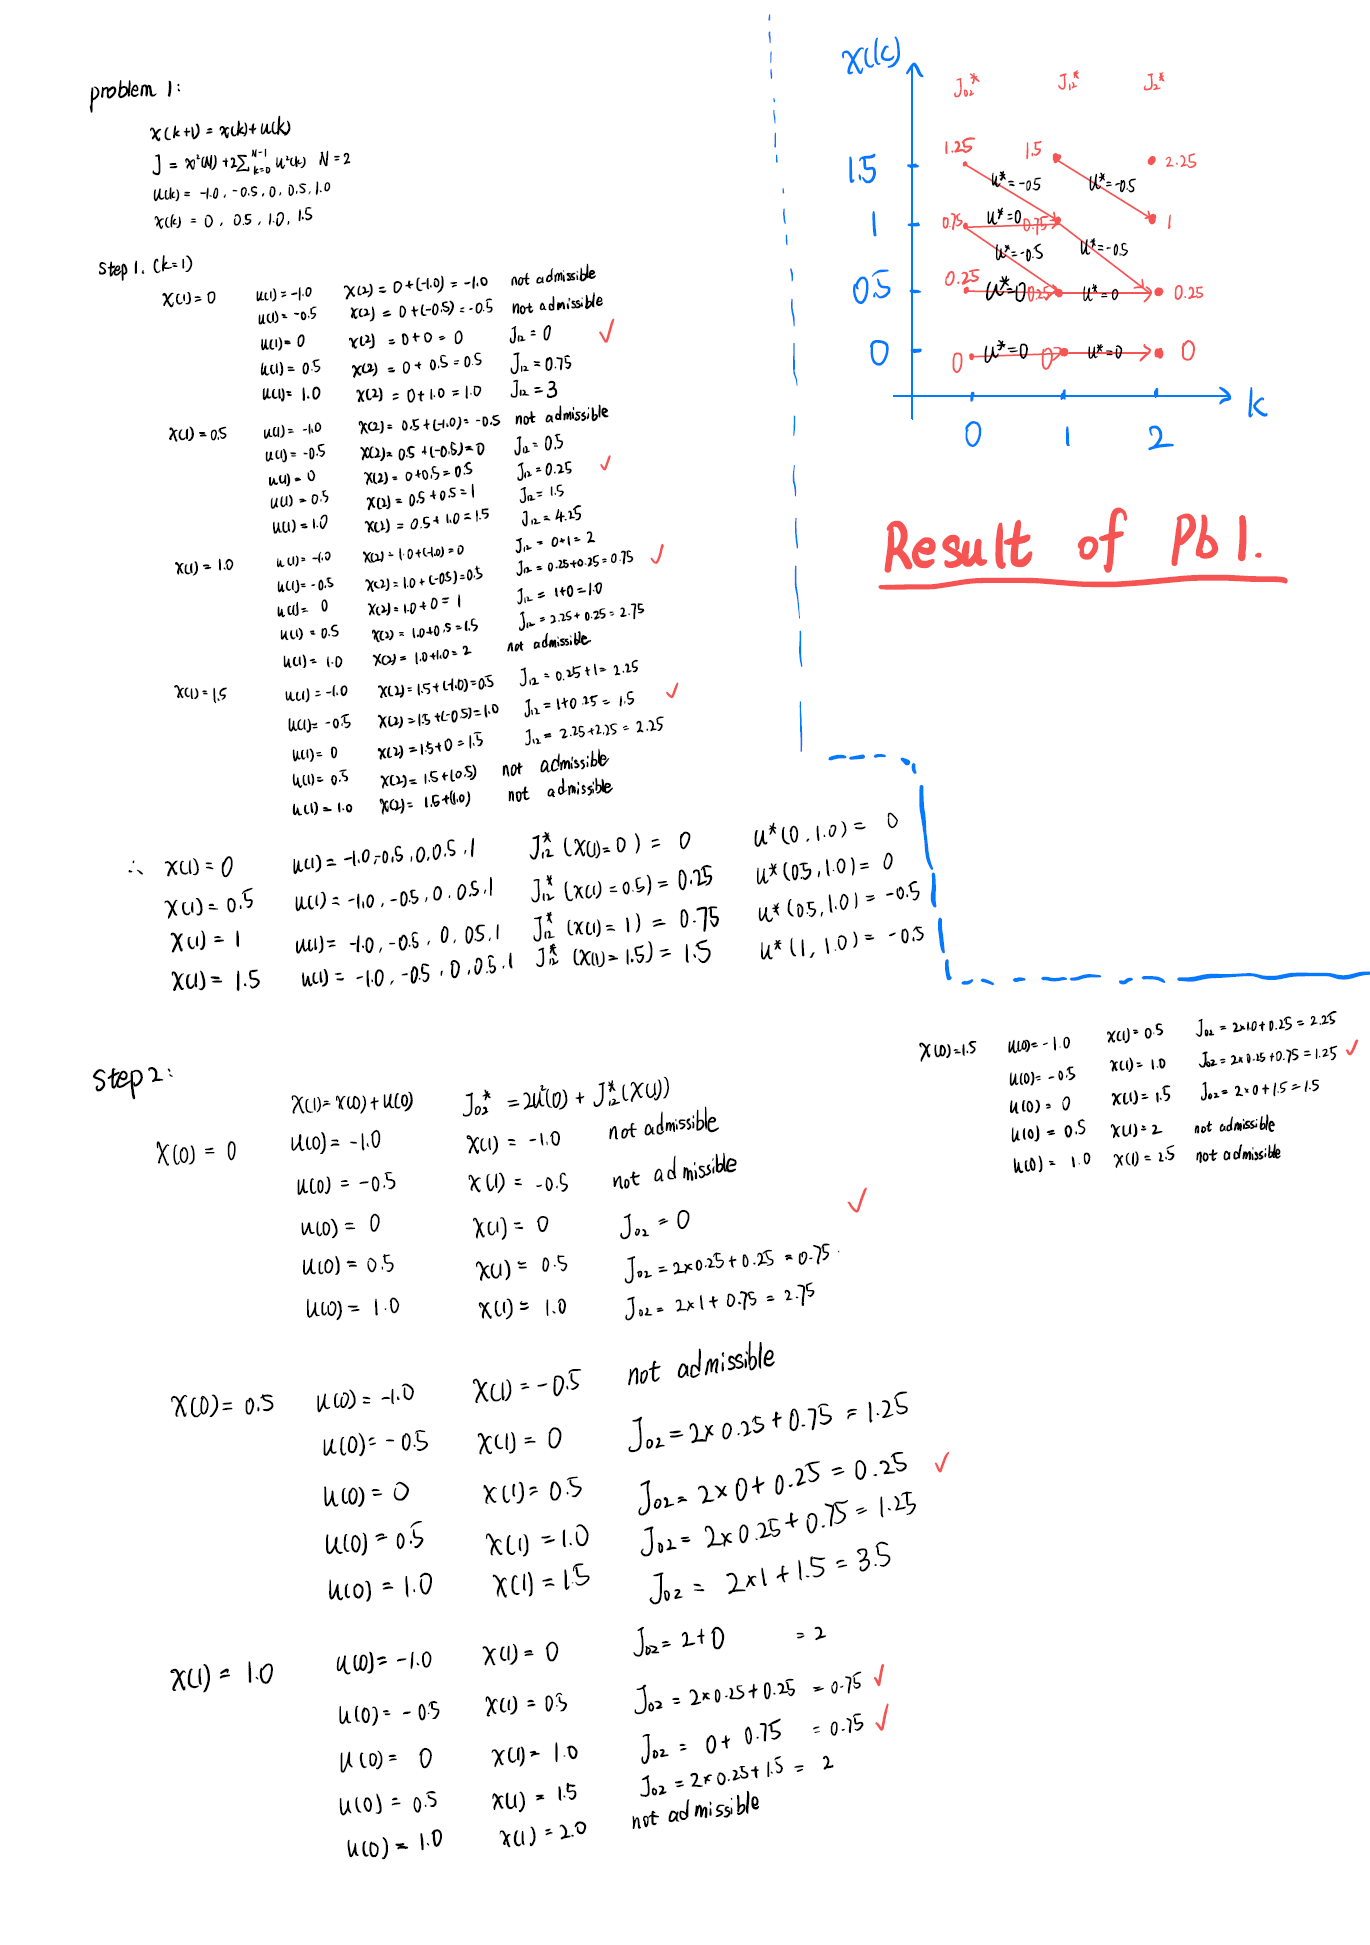
\includegraphics[width=0.7\textwidth]{graph 1.png}
    \caption{Graph 1}\label{fig:pb1graph1}
\end{figure}

According to the Figure \ref{fig:pb1graph1}, the best input is:

\section{Problem 2}
\section{Problem 3}
% insert 4 pictures here
\begin{figure}[h!]
    \centering
    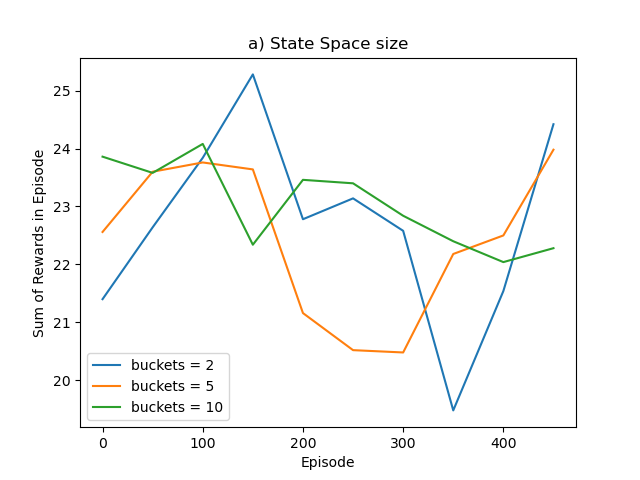
\includegraphics[width=0.7\textwidth]{graph a.png}
    \caption{Graph 1}
\end{figure}
\begin{figure}[h!]
    \centering
    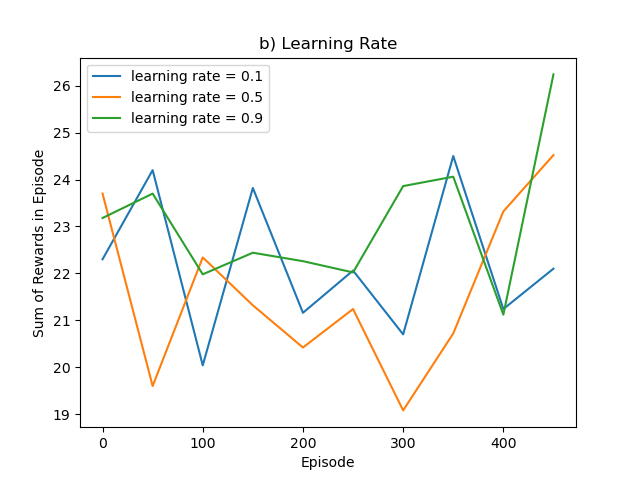
\includegraphics[width=0.7\textwidth]{graph b.png}
    \caption{Graph 1}
\end{figure}
\begin{figure}[h!]
    \centering
    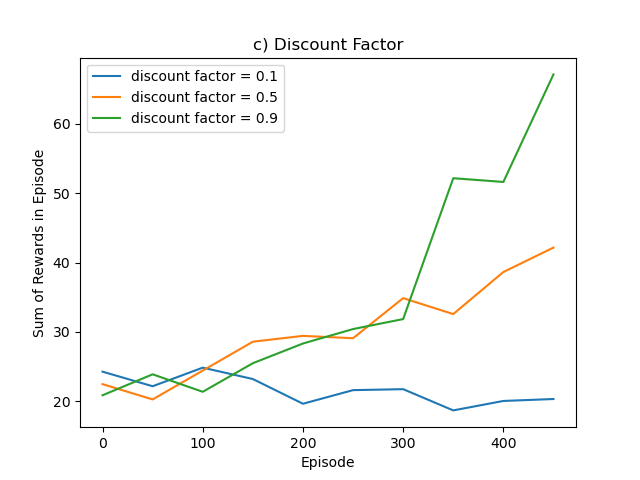
\includegraphics[width=0.7\textwidth]{graph c.png}
    \caption{Graph 1}
\end{figure}
\begin{figure}[h!]
    \centering
    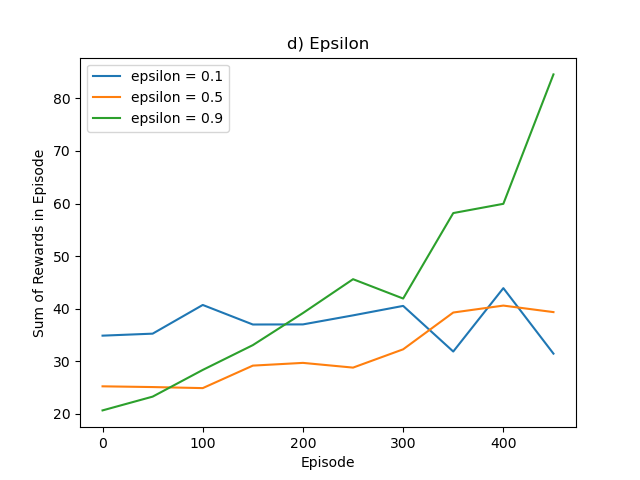
\includegraphics[width=0.7\textwidth]{graph d.png}
    \caption{Graph 1}
\end{figure}

\end{document}